\documentclass[a4paper,12pt]{article}
\usepackage[utf8x]{inputenc}
\usepackage[english]{babel}
\usepackage[T1]{fontenc}
\usepackage{times}
\usepackage{graphicx}
\usepackage{float}
\usepackage{subfig}
\usepackage[top=2cm, bottom=2cm, left=2.5cm, right=2.5cm]{geometry}

\batchmode

\title{\Huge{Hildo Brilleman's Social Network}}
\date{\today}

\begin{document}
\pagenumbering{gobble}
\clearpage
\thispagestyle{empty}

\maketitle


\begin{figure}[H]
\centering
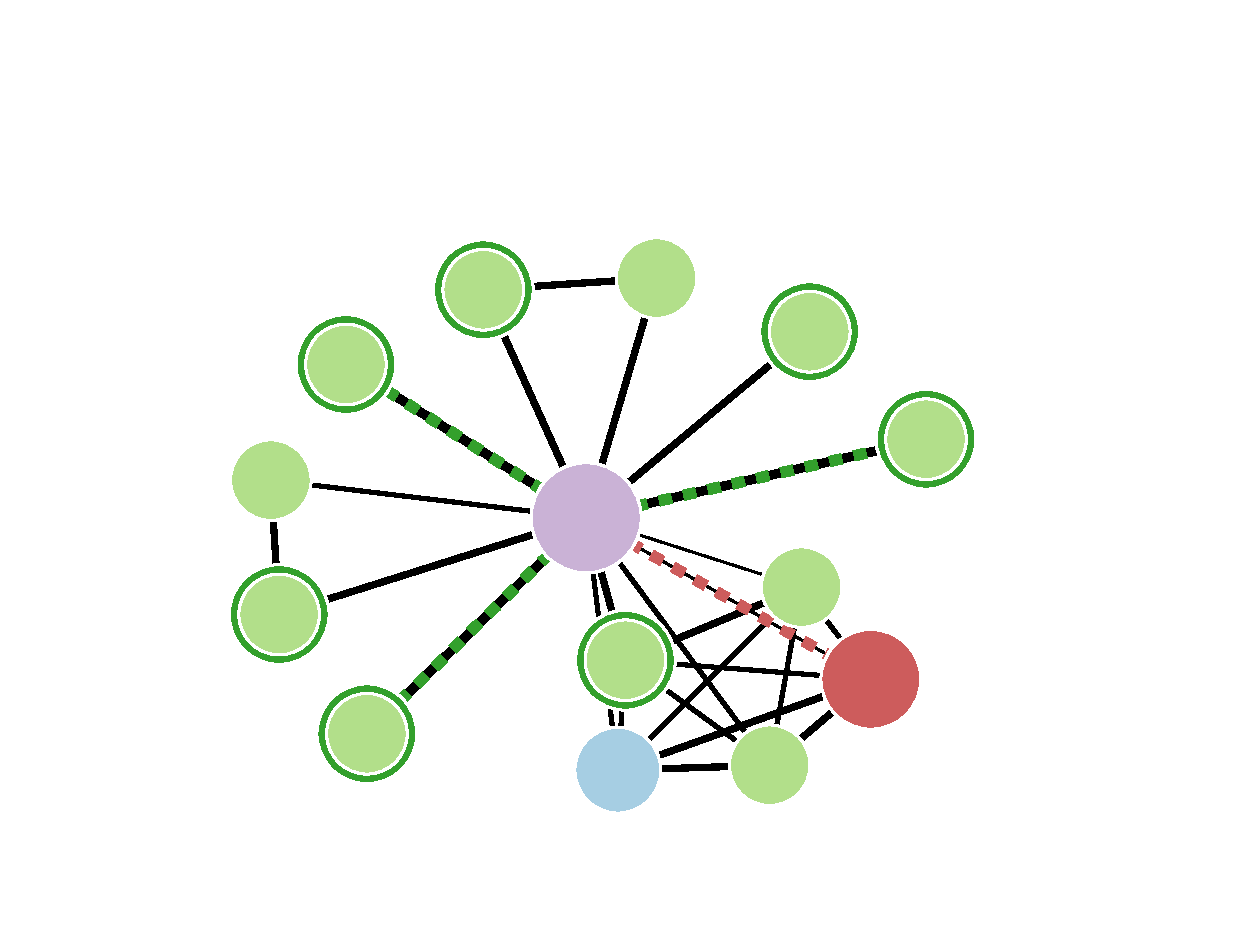
\includegraphics[scale=0.9]{ilcavi87/egosite/egonet/static/egonet/report/sample_net}
\end{figure}


\begin{center}
\Large{\textbf{Advanced Management Program SPRING M4 2017}}


\begin{figure}[H]
\centering

\includegraphics[scale=0.2]{/home/networker/webapps/netwrkr/networker/egonet/../media/logos/iese_logo}
\end{figure}

\small{}
\end{center}

\newpage
\clearpage
\pagenumbering{arabic}


\section*{Why your social network matters}


Thinking about your social network might help you go beyond a simplistic view of what your contacts are ---who do you know?--- and help you think about how the people in your company are connected to each other. These connections are a key defining element of any human group. Understanding how people relate to each other is of capital importance for managers and leaders. Note that connections among people in a firm go beyond its formal hierarchy of who reports to whom. The informal relations of advise, support, friendship and antagonism, generate an informal network of relations among people that shapes, in part, how information spreads; and can facilitate, or hinder, consensus and coordinated action.

Social scientists define the social structure of a group as the repeated patterns of relations among the people that compose it. The patterns of relations among people in your company ---its social structure---, and your concrete position in those patterns, might allow you to access and procure valuable intangible assets, such as good advice, technical knowledge, emotional support, etc. The concept of social capital captures the fact that some people have an advantage only because of their position in the social structure of a group.


\begin{figure}[H]
\centering
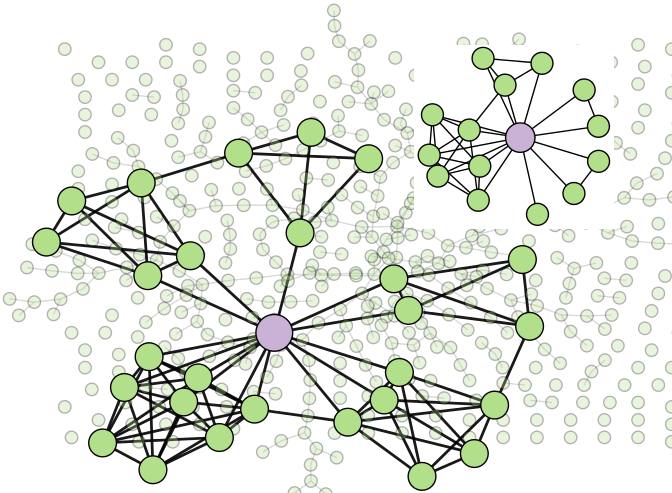
\includegraphics[scale=0.7]{ilcavi87/egosite/egonet/static/egonet/report/organizational_network}
\caption{This plot illustrates a broker (the purple node) embedded in an organizational network. The broker links several densely connected groups, that would be disconnected if it weren't for the broker's connections. The inset depicts the personal social network of the broker, with contacts from several groups that are not connected among them.}
\end{figure}


A very common pattern of relations in informal networks is the presence of groups with dense internal connections ---called clusters---, linked by a few ties between people of different groups. Inside a cluster everybody is directly linked to almost everybody else. The cohesion of clusters fosters the development of trust among its members, which allows fast decision making and reduces coordination costs for action. The links among clusters, that is the links among persons of different clusters, can be conceptualized as bridges that allow information and resources flow among parts of the organization that would be far apart if there were no such bridging links. Thus, bridges are key for achieving fast decision making and effective coordinated action at the organization level, and not only inside the small groups that form its informal social network.

In actual organizations, such as your company, the presence of bridge links among different informal groups will emerge spontaneously to some degree. However, fast decision making and effective coordinated action, especially in high uncertainty conditions, can only be achieved if conscious action reinforces the spontaneous tendency of bridges among groups to emerge. Therefore, a key aspect of leadership skills is learn to build social relations that act as bridges across groups.

At the individual level, social science research has consistently shown that individuals that have social connections that span more than one densely connected cluster ---a broker--- achieve better career outcomes, and more importantly, are a source of good and innovative ideas that usually benefit the whole organization.

You have to think about your professional social network taking into account the big picture of the structure of the groups in which you are embedded. We designed this report with this goal in mind. The report is based on the confidential information on your social network collected with the web-based survey that you completed. The goal of this report is to help you evaluate how your professional social network may allow you access to important assets that will help you achieve your professional goals. To improve the interpretation of your results, we compare them with the results of the other people in your group.

The report is organized in three parts. First, we analyze your network in terms of the number and the diversity of your contacts. Second, we analyze your network in terms of the kind and the strength of the relationships between you and your contacts. Third, we analyze the structure of your network, focusing on the patterns of relations among your contacts.


\newpage


\section*{Your Contacts}


The characteristics of the people to whom you are directly related, that is, their gender, age, rank, etc ... are the attributes of your contacts. The diversity of the attributes of the people that form your personal social network is a source of different perspectives that can allow you to find innovative solutions to the problems that you face at work. People with different attributes are likely to try different approaches in a wide variety of problems. This can allow a diverse group to find an innovative solution to a common problem. However, attribute diversity among people in your network might also hamper deliberation and mutual understanding. Diversity increases coordination costs, and thus it can hinder action and decision making if the group is not able to deal with conflict and disagreement among members.

The following figures depict the distribution, for your own social network and for the whole reference group, of 5 important attributes: gender, age, workplace, rank, and functional area inside their firm.


\begin{figure}[H]
\centering
\subfloat[Average of your group results]{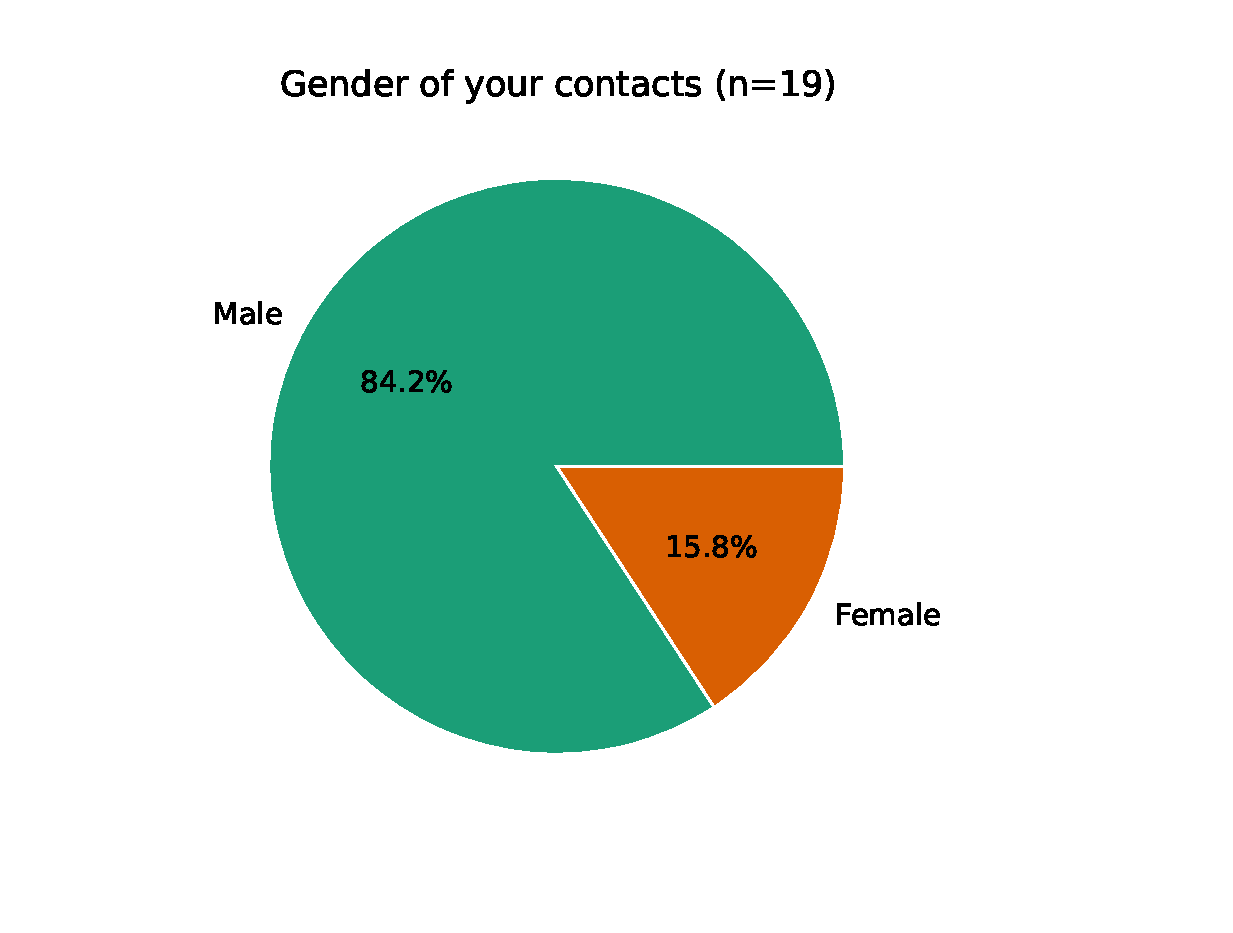
\includegraphics[scale=0.3]{/home/networker/webapps/netwrkr/networker/media/egoreports/3_145721a8-a107-4fd8-a23b-49ab6483bbd0/average/gender}}
\hspace{.01in}
\subfloat[Your personal results]{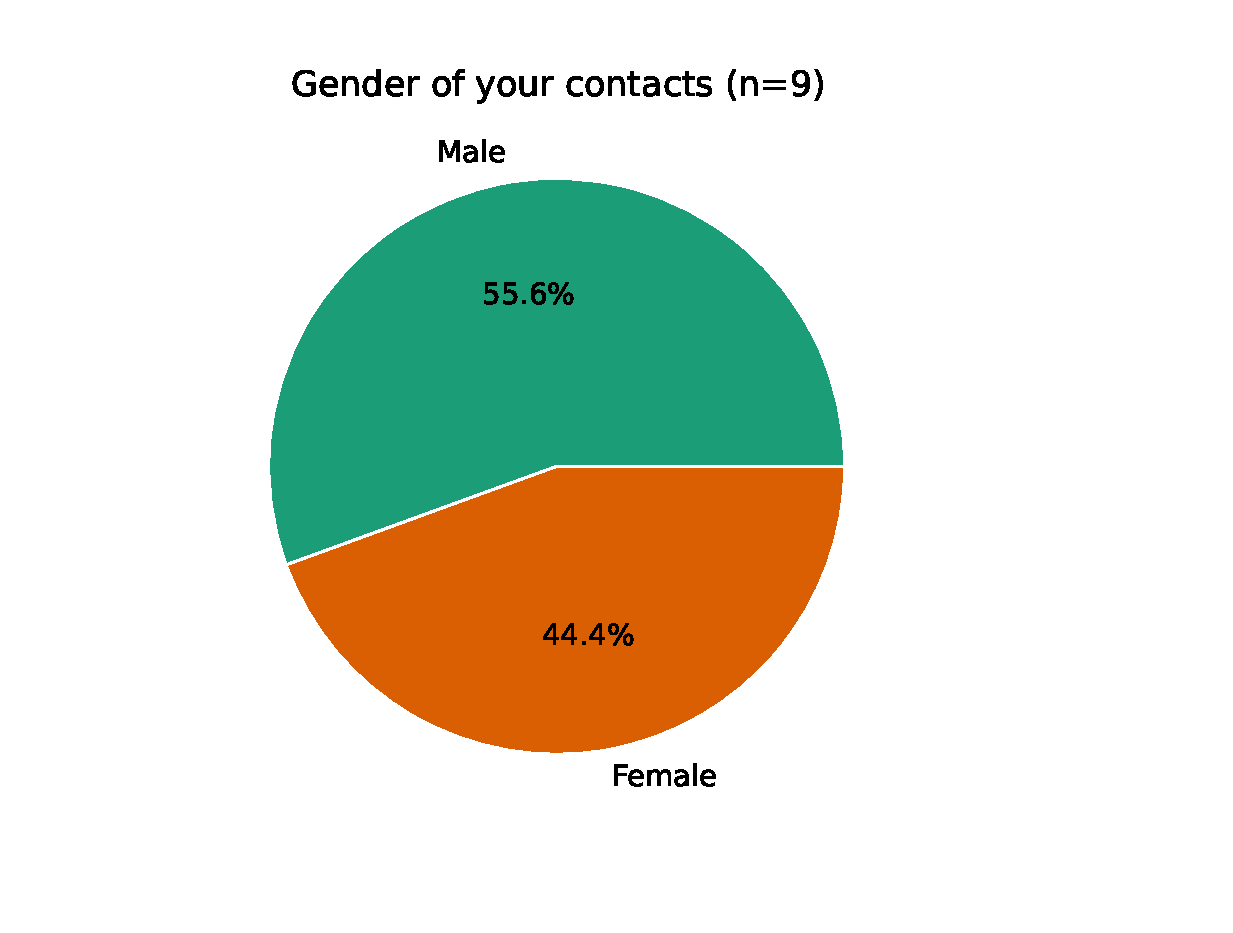
\includegraphics[scale=0.3]{/home/networker/webapps/netwrkr/networker/media/egoreports/3_145721a8-a107-4fd8-a23b-49ab6483bbd0/40dd7ad9-ebed-4bd8-9ab0-034943da2936/gr_gender}}
\caption{This chart shows the gender distribution of your contacts. Gender diversity reveals your exposure to the view-points and experiences of the different sexes. This is partly defined by demographics since there are still significantly more men than women in most business settings. But it can be also driven by stereotypes: some men may find it difficult to build good professional relationships with women (and vice-versa).}
\end{figure}


\begin{figure}[H]
\centering
\subfloat[Average of your group results]{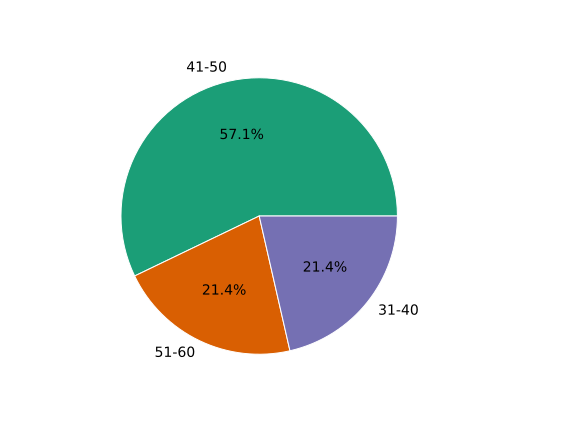
\includegraphics[scale=0.3]{/home/networker/webapps/netwrkr/networker/media/egoreports/3_145721a8-a107-4fd8-a23b-49ab6483bbd0/average/age}}
\hspace{.01in}
\subfloat[Your personal results]{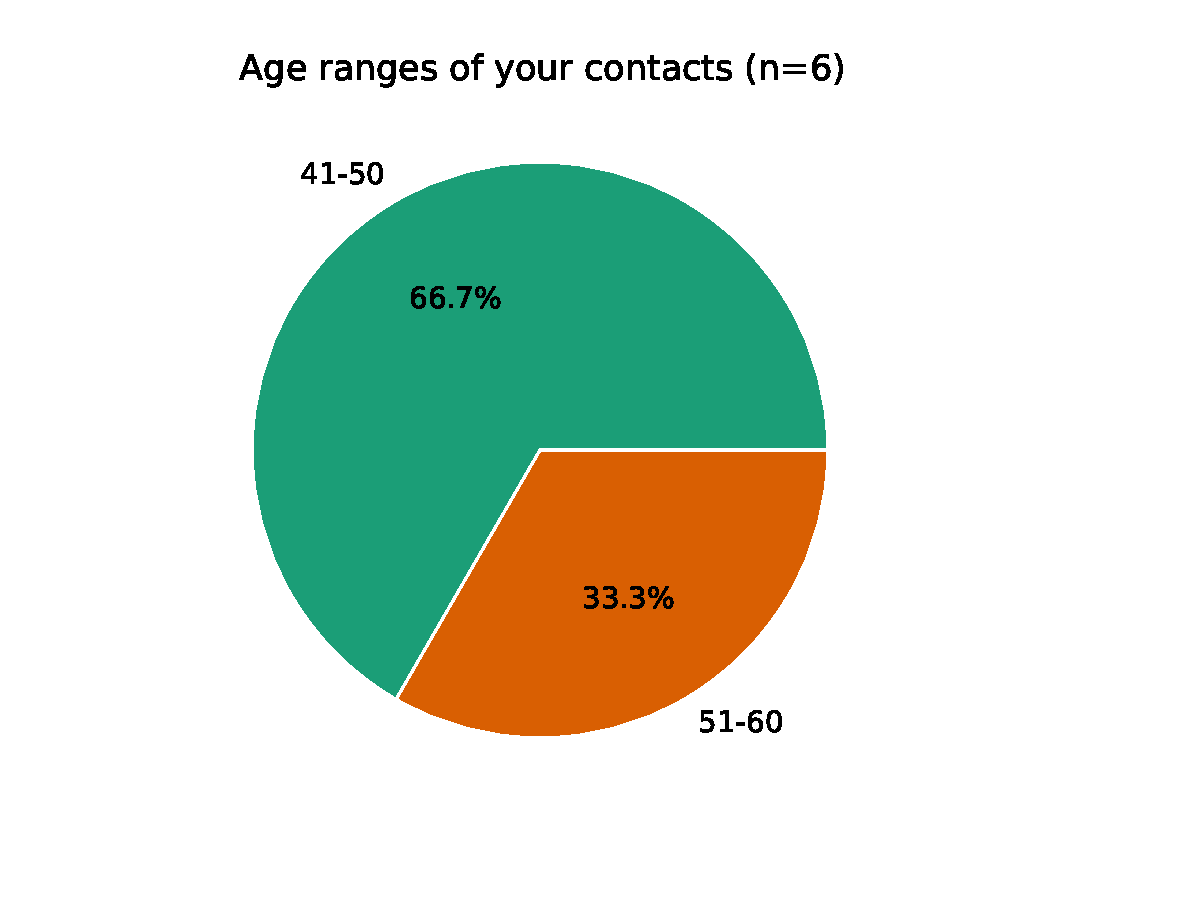
\includegraphics[scale=0.3]{/home/networker/webapps/netwrkr/networker/media/egoreports/3_145721a8-a107-4fd8-a23b-49ab6483bbd0/40dd7ad9-ebed-4bd8-9ab0-034943da2936/gr_age}}
\caption{This graph illustrates the distribution of your contacts by age. The age of your contacts is important because different generations have gone through different experiences that configure their opinions and their attitudes. The age of our contacts typically increases with age. This is natural, but also has draw-backs. A network can be a bridge across generations or it may amplify the natural separation between them.}
\end{figure}


\begin{figure}[H]
\centering
\subfloat[Average of your group results]{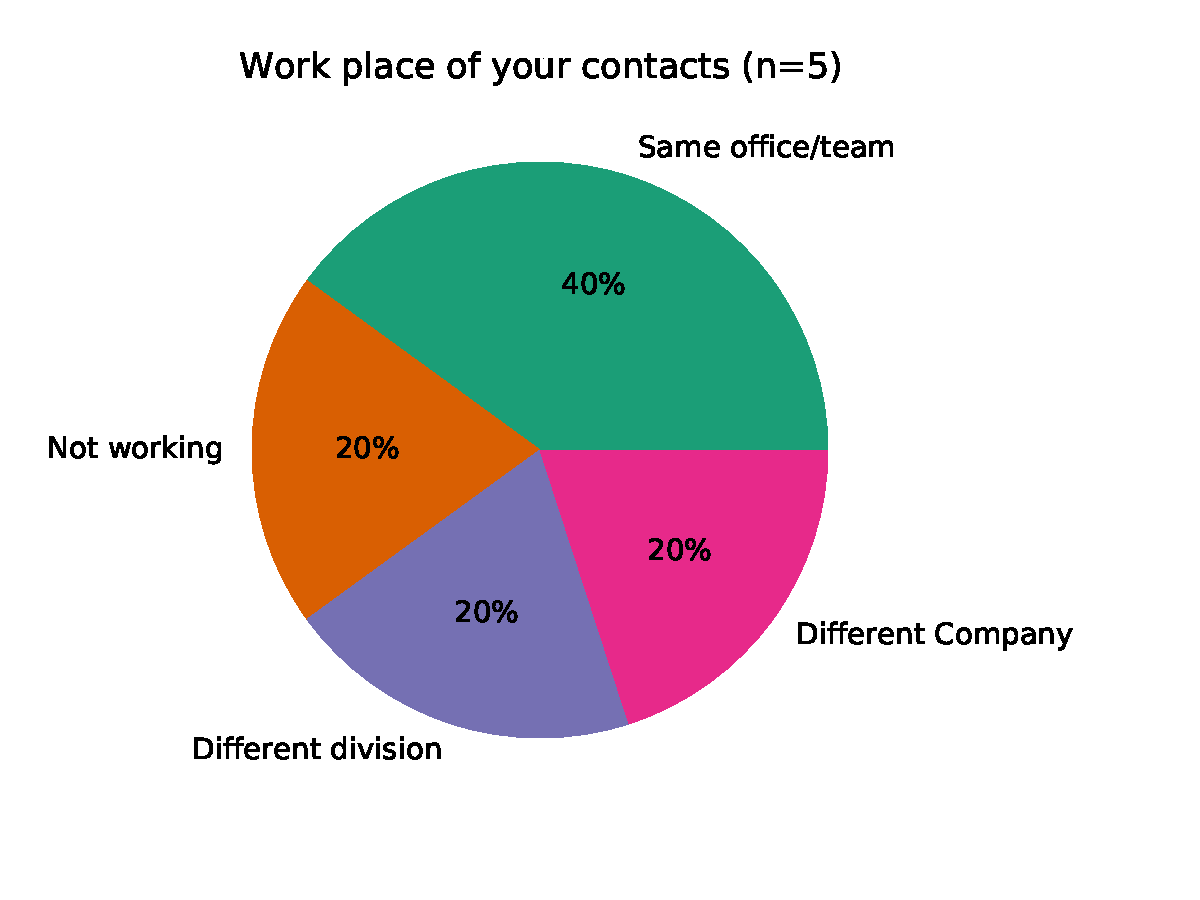
\includegraphics[scale=0.3]{/home/networker/webapps/netwrkr/networker/media/egoreports/3_145721a8-a107-4fd8-a23b-49ab6483bbd0/average/work}}
\hspace{.01in}
\subfloat[Your personal results]{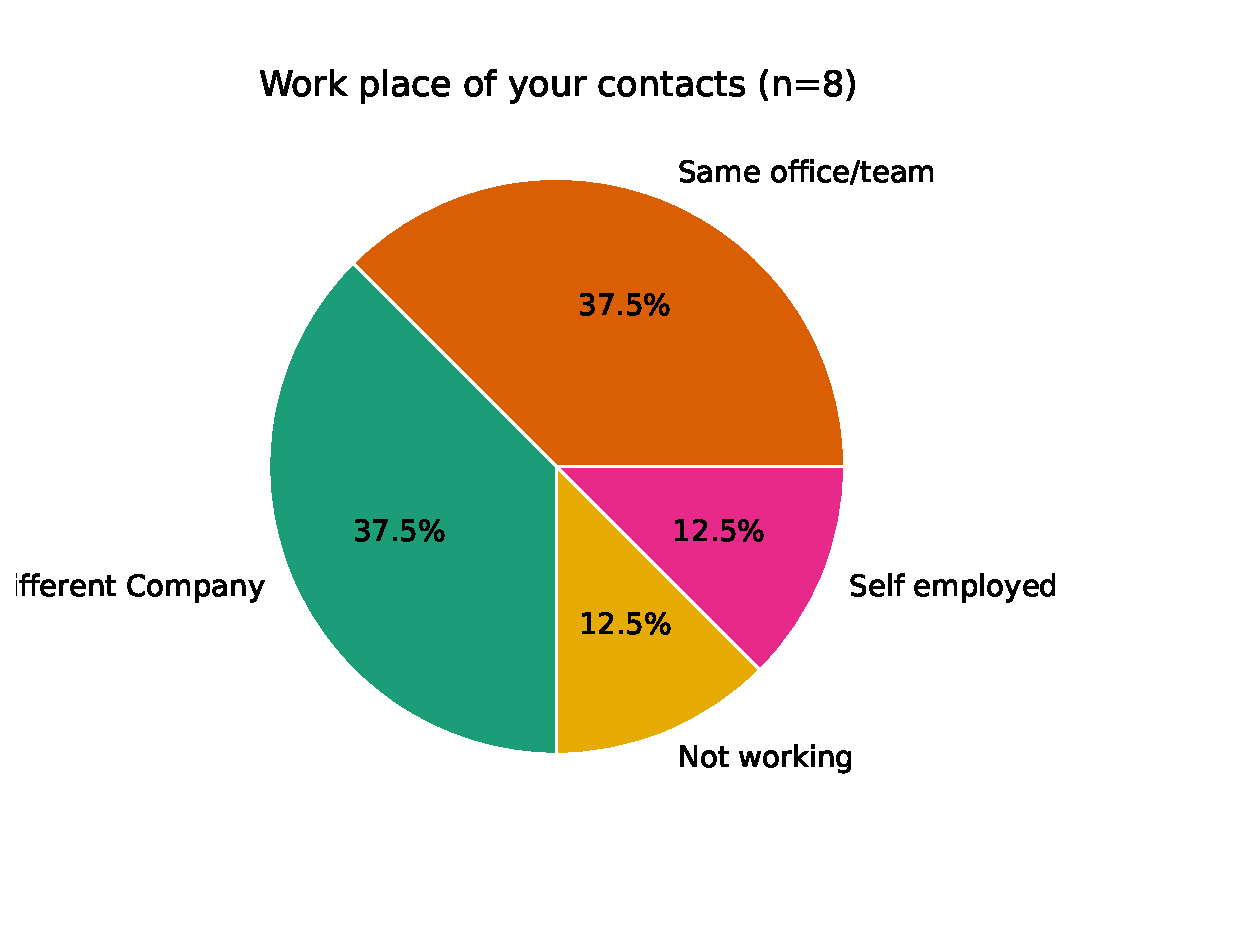
\includegraphics[scale=0.3]{/home/networker/webapps/netwrkr/networker/media/egoreports/3_145721a8-a107-4fd8-a23b-49ab6483bbd0/40dd7ad9-ebed-4bd8-9ab0-034943da2936/gr_work}}
\caption{The graph above shows the proportion of contacts working in your same unit, in your same function (but in a different unit), in your same firm (but in a different function), and in other firms. It indicates the extent to which your network is limited to your own firm or office.}
\end{figure}


\begin{figure}[H]
\centering
\subfloat[Average of your group results]{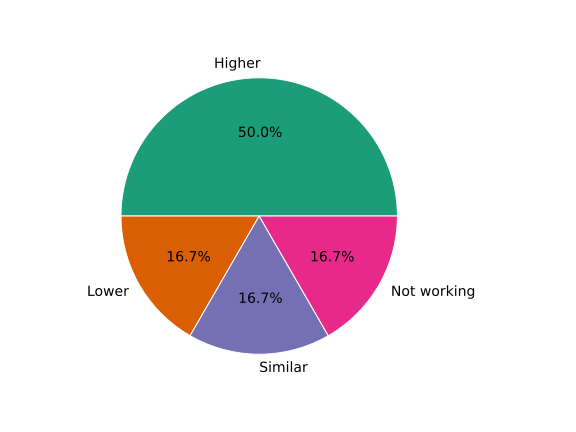
\includegraphics[scale=0.3]{/home/networker/webapps/netwrkr/networker/media/egoreports/3_145721a8-a107-4fd8-a23b-49ab6483bbd0/average/rank}}
\hspace{.01in}
\subfloat[Your personal results]{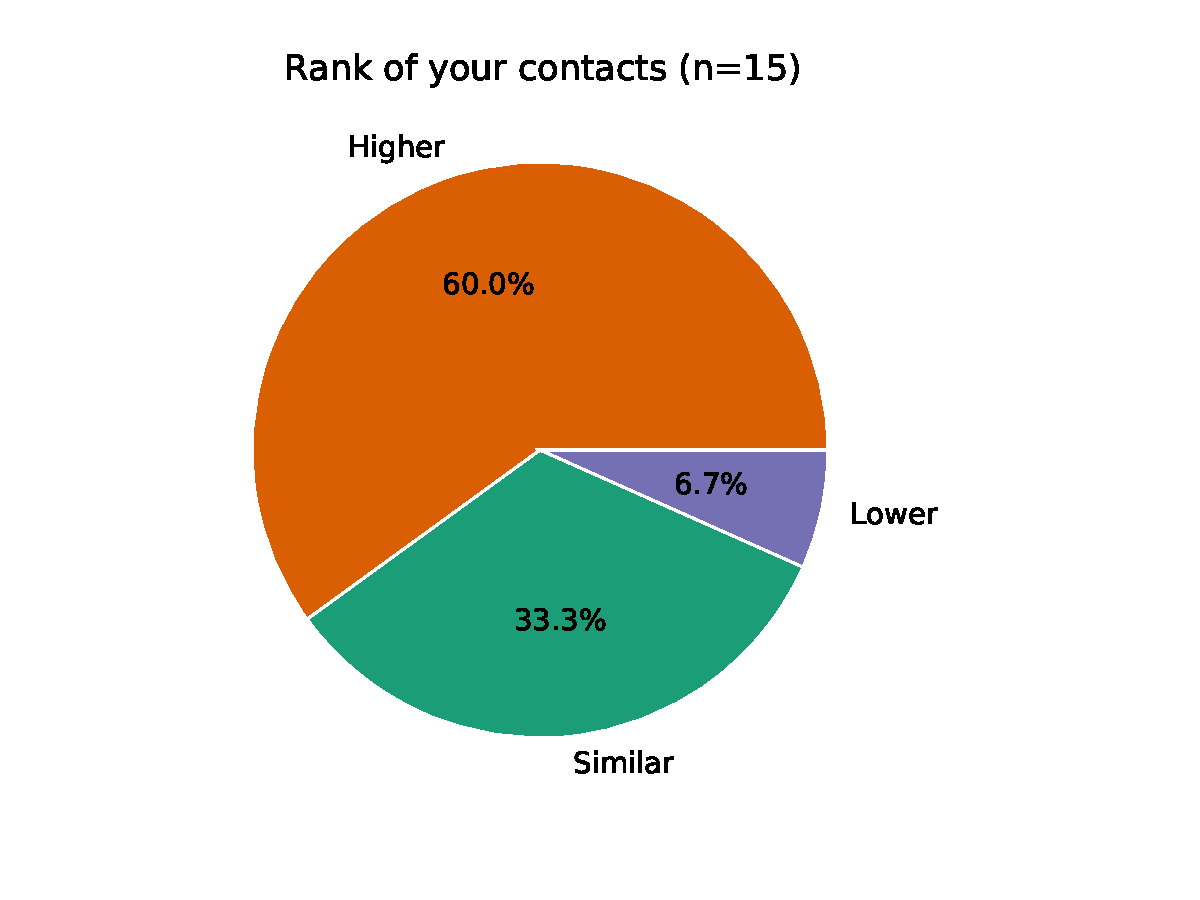
\includegraphics[scale=0.3]{/home/networker/webapps/netwrkr/networker/media/egoreports/3_145721a8-a107-4fd8-a23b-49ab6483bbd0/40dd7ad9-ebed-4bd8-9ab0-034943da2936/gr_rank}}
\caption{The chart looks at the hierarchical diversity of your network. The diversity is your network in terms of rank is partly dependent on your own rank.}
\end{figure}


\begin{figure}[H]
\centering
\subfloat[Average of your group results]{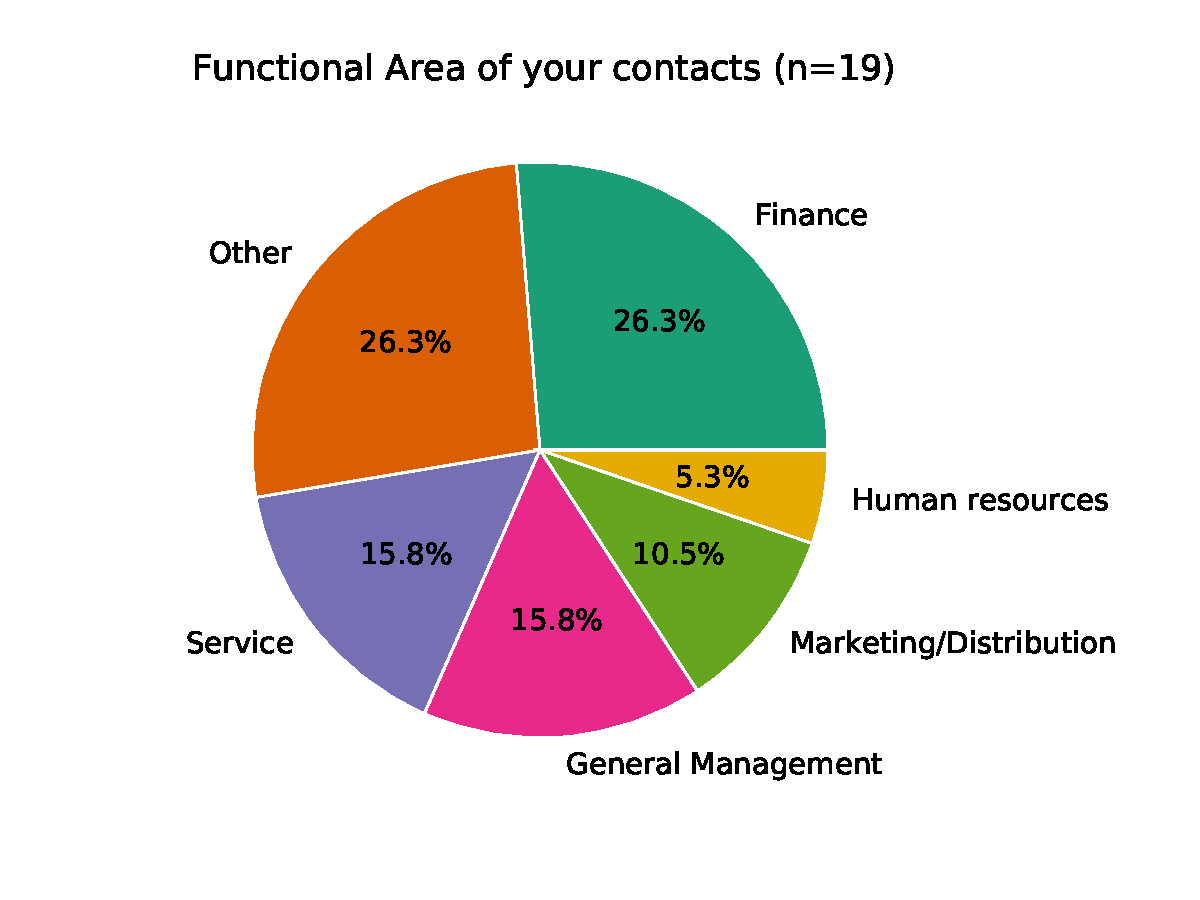
\includegraphics[scale=0.3]{/home/networker/webapps/netwrkr/networker/media/egoreports/3_145721a8-a107-4fd8-a23b-49ab6483bbd0/average/functional_area}}
\hspace{.01in}
\subfloat[Your personal results]{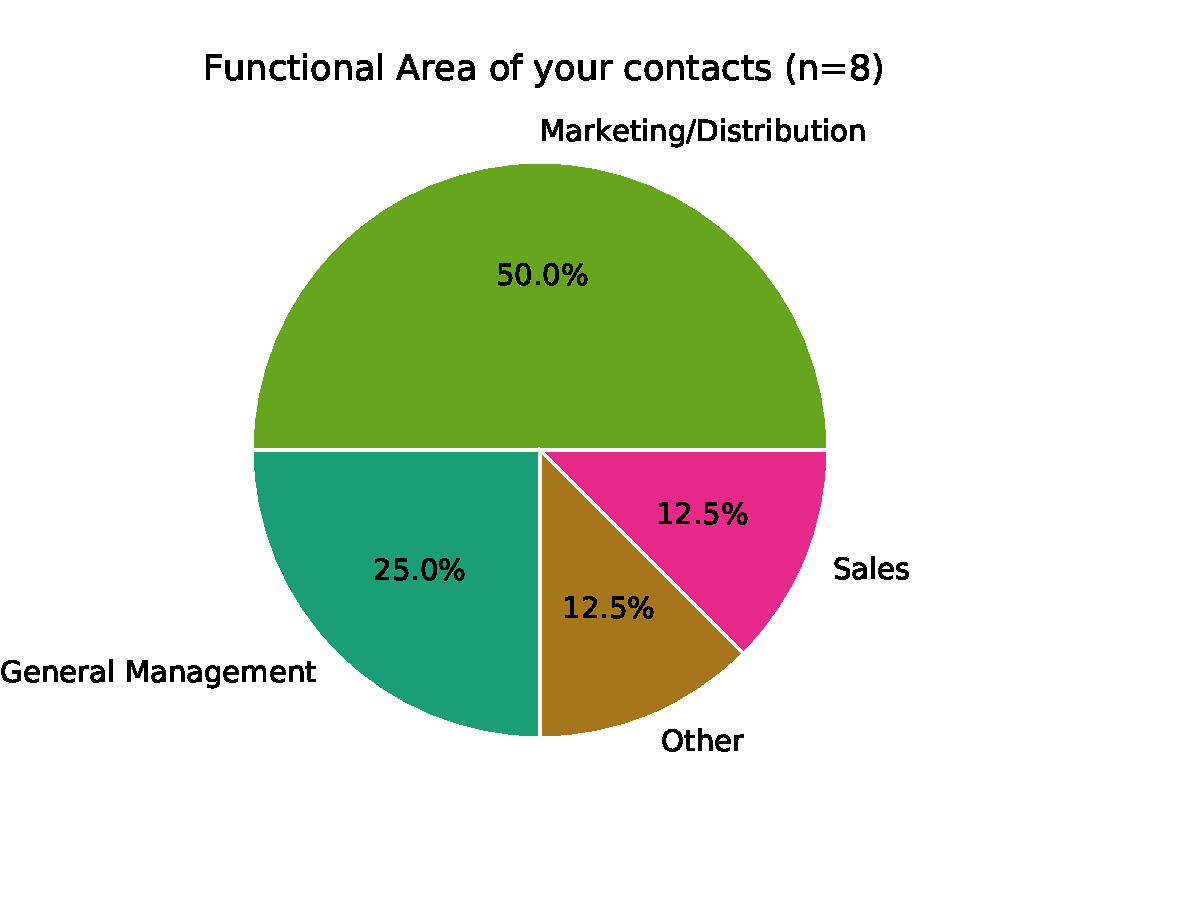
\includegraphics[scale=0.3]{/home/networker/webapps/netwrkr/networker/media/egoreports/3_145721a8-a107-4fd8-a23b-49ab6483bbd0/40dd7ad9-ebed-4bd8-9ab0-034943da2936/gr_functional_area}}
\caption{This graph illustrates the distribution of your contacts by their primary functional or professional area. It measures the extent to which your network reaches across functional boundaries. A network with contacts from different functional backgrounds exposes you to a richer picture of the business and allows you to learn about more opportunities to achieve your professional goals.}
\end{figure}


\section*{Your Relations}


The strength and quality of the relationships between you and your contacts is a good proxy of their willingness to help, and their diversity affects the extent of the resources and information they can provide. The disposition to help and the breadth of that help may be also shaped by the structure of your network.

Of course, relationships are multidimensional and there are many possible definitions of strength and quality. Strength is a combination of mutual trust, frequency of interaction and common contacts. Quality is a combination of the help they provide, both at the personal and professional level, and also mutual trust and respect. The following figures depict several dimensions of the strength and quality of relations: how close they are in terms of mutual trust, the frequency of interactions, the help they provide, and the context in which the relationship was established.


\begin{figure}[H]
\centering
\subfloat[Average of your group results]{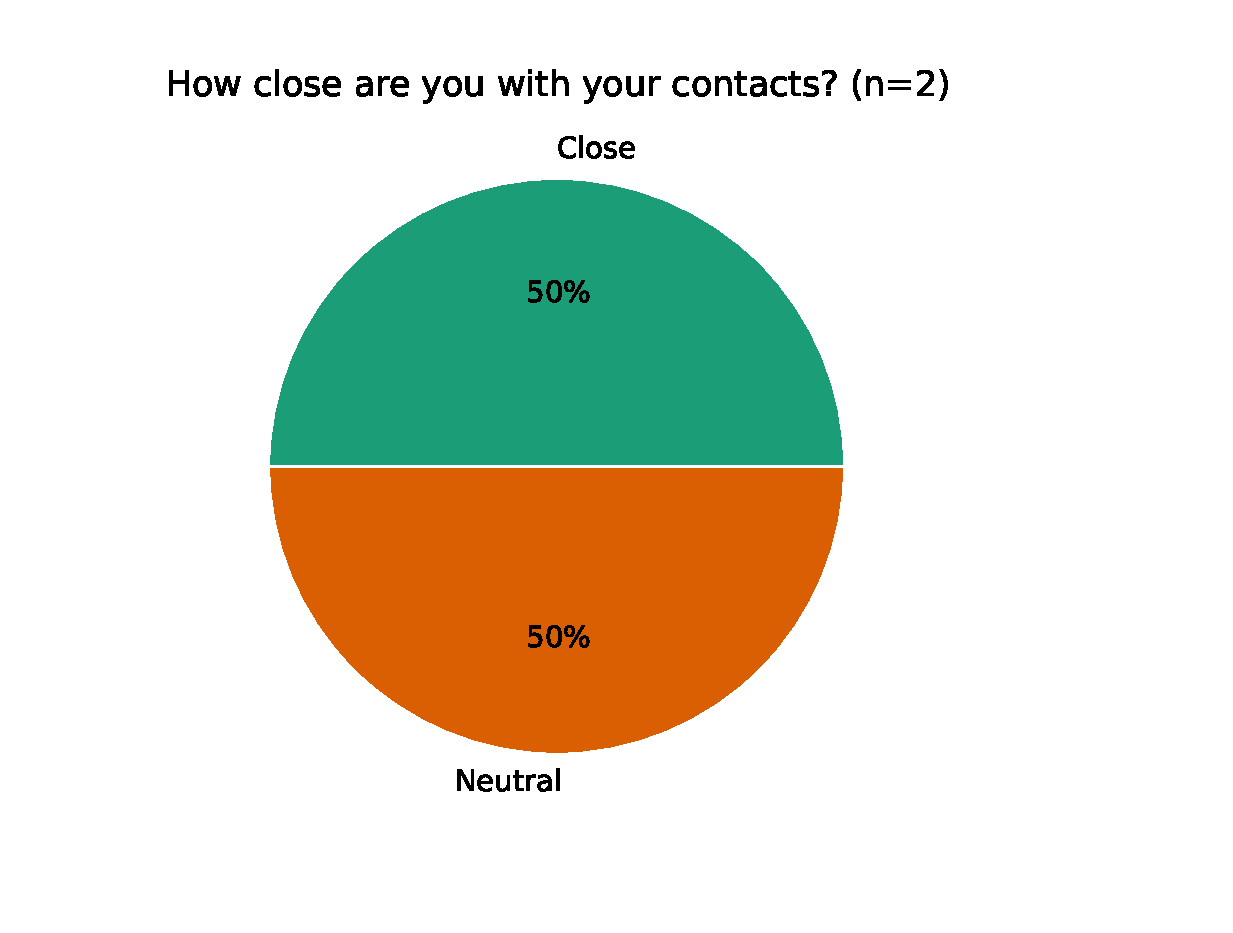
\includegraphics[scale=0.3]{/home/networker/webapps/netwrkr/networker/media/egoreports/3_145721a8-a107-4fd8-a23b-49ab6483bbd0/average/strength}}
\hspace{.01in}
\subfloat[Your personal results]{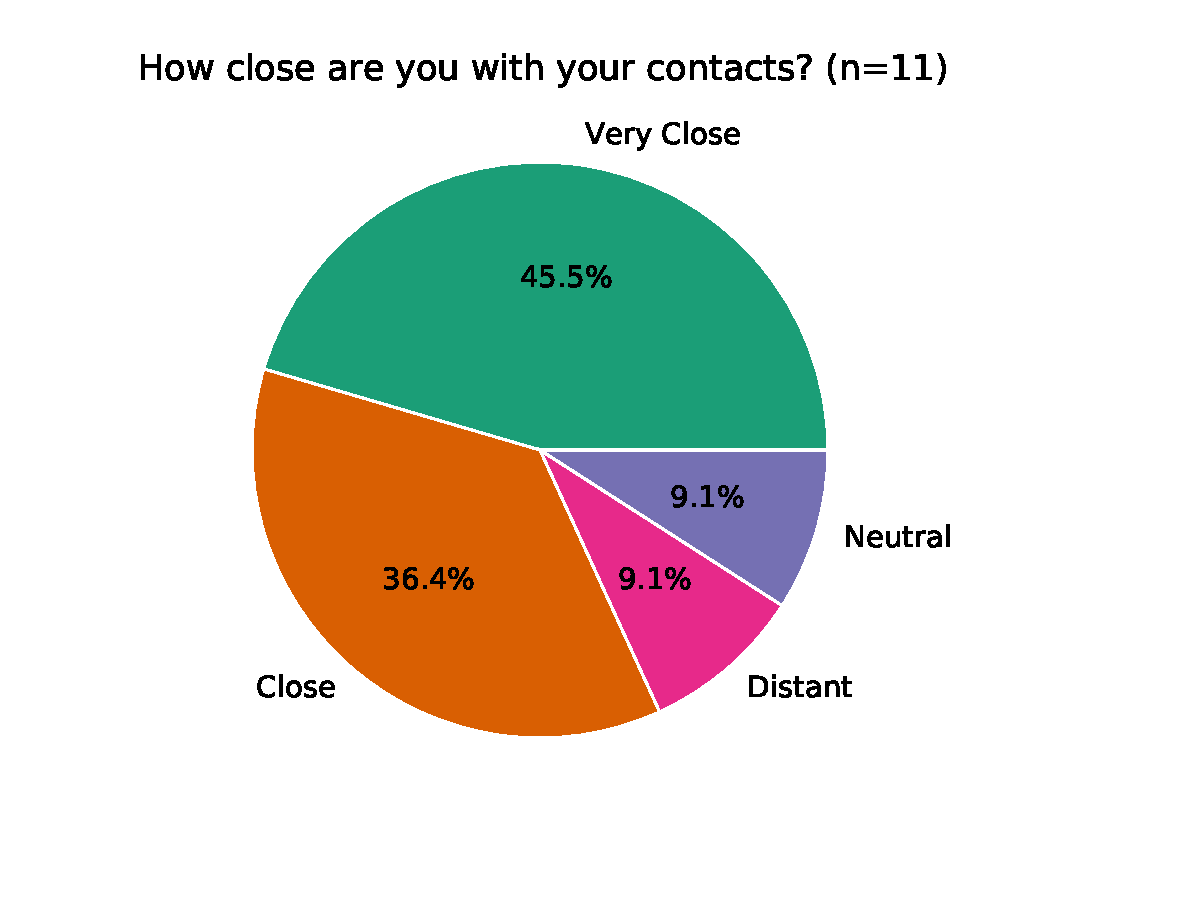
\includegraphics[scale=0.3]{/home/networker/webapps/netwrkr/networker/media/egoreports/3_145721a8-a107-4fd8-a23b-49ab6483bbd0/40dd7ad9-ebed-4bd8-9ab0-034943da2936/gr_strength}}
\caption{This graph represents the strength of the relationship with each contact in term of the closeness between you and the contact. Closer relationships might help you receive more support from your contacts.}
\end{figure}


\begin{figure}[H]
\centering
\subfloat[Average of your group results]{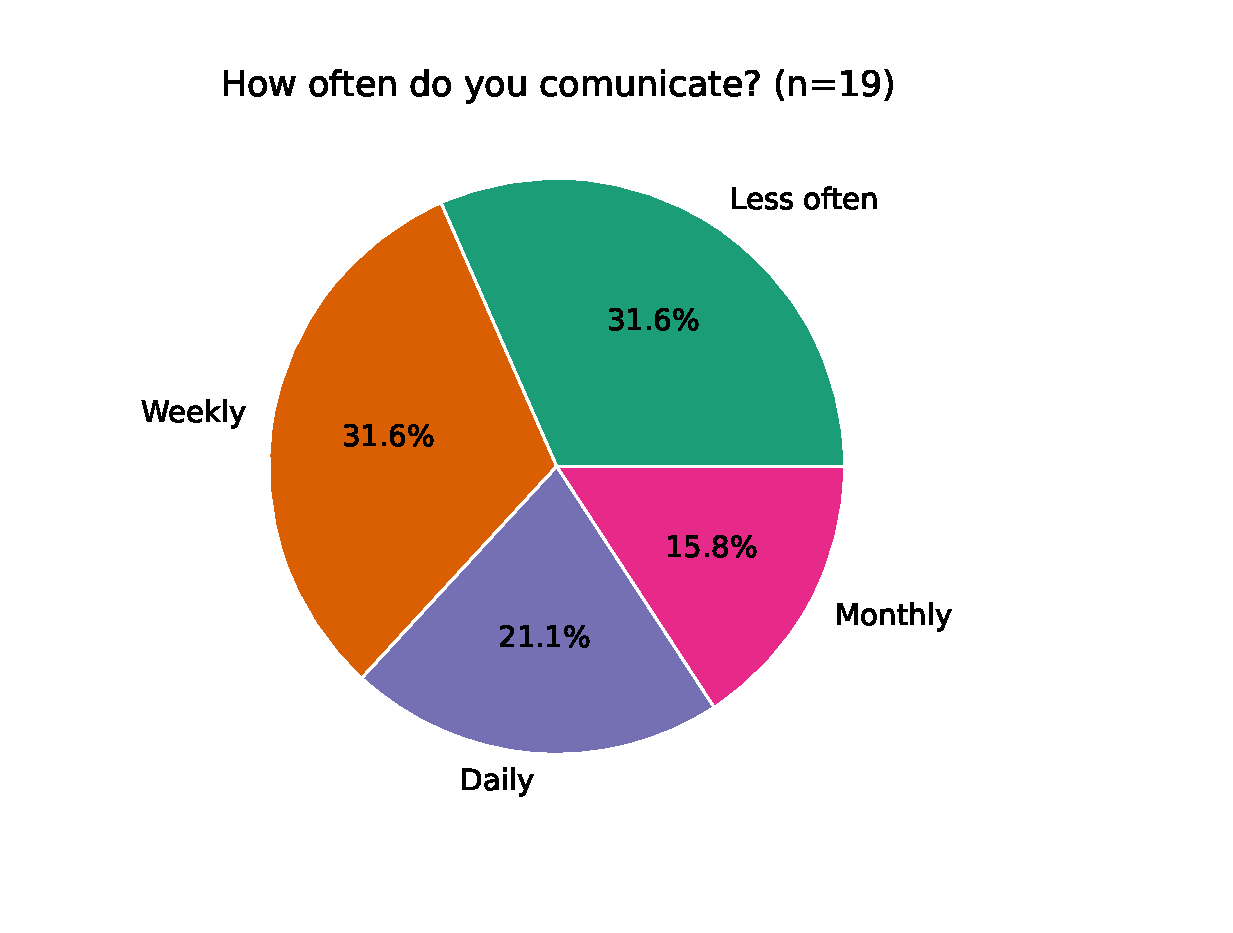
\includegraphics[scale=0.3]{/home/networker/webapps/netwrkr/networker/media/egoreports/3_145721a8-a107-4fd8-a23b-49ab6483bbd0/average/frequency}}
\hspace{.01in}
\subfloat[Your personal results]{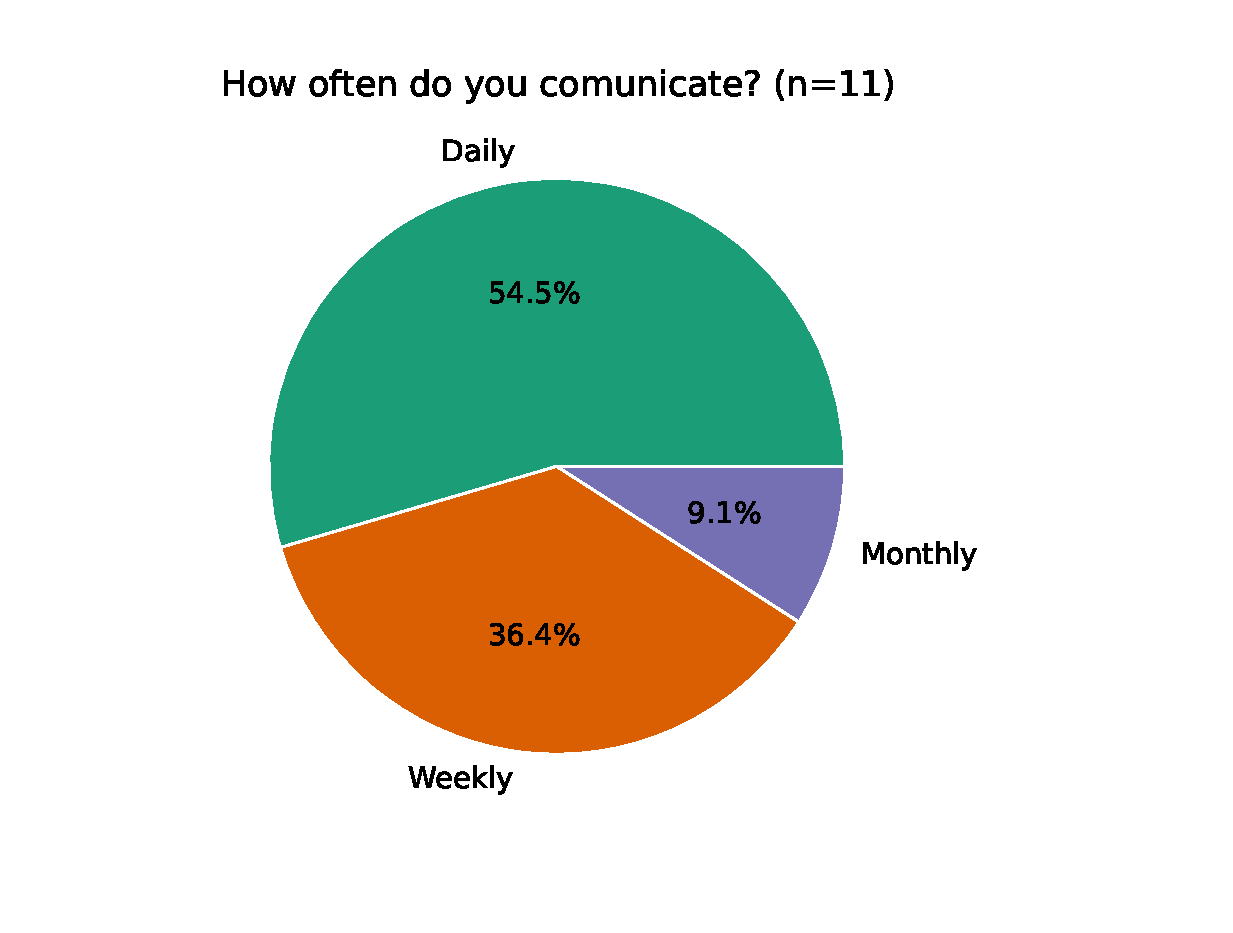
\includegraphics[scale=0.3]{/home/networker/webapps/netwrkr/networker/media/egoreports/3_145721a8-a107-4fd8-a23b-49ab6483bbd0/40dd7ad9-ebed-4bd8-9ab0-034943da2936/gr_frequency}}
\caption{The chart displays the frequency with which you communicate with your contacts capturing your tendency to concentrate this communication on a specific time frame (e.g., on a weekly basis).}
\end{figure}


\begin{figure}[H]
\centering
\subfloat[Average of your group results]{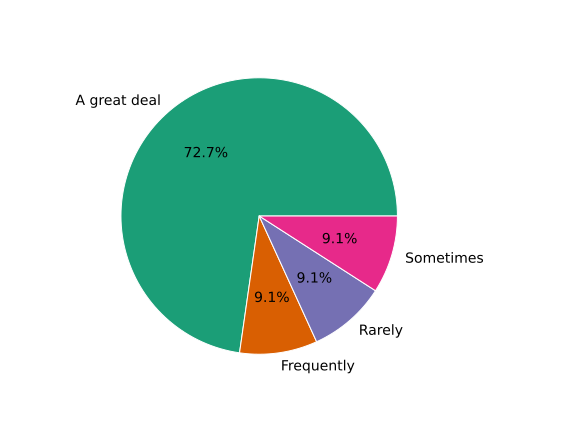
\includegraphics[scale=0.3]{/home/networker/webapps/netwrkr/networker/media/egoreports/3_145721a8-a107-4fd8-a23b-49ab6483bbd0/average/helps}}
\hspace{.01in}
\subfloat[Your personal results]{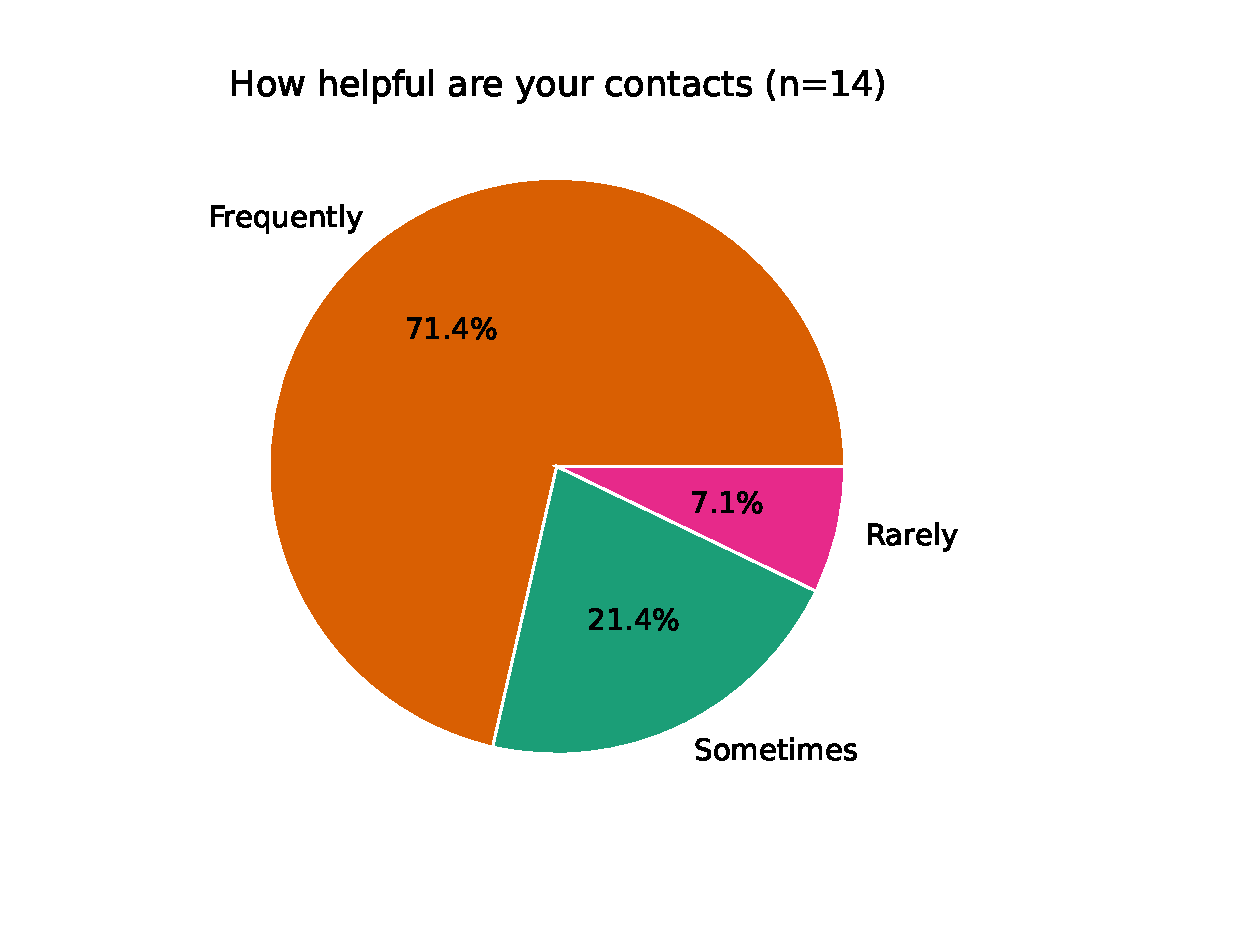
\includegraphics[scale=0.3]{/home/networker/webapps/netwrkr/networker/media/egoreports/3_145721a8-a107-4fd8-a23b-49ab6483bbd0/40dd7ad9-ebed-4bd8-9ab0-034943da2936/gr_helps}}
\caption{This graph represents how helpful your contacts are and the degree of supportiveness. Contacts with whom you have a long-lasting, frequent, and emotionally close relationship know you and your needs well. They are around to help when you need it, and they are more inclined to do so than weakly tied contacts.}
\end{figure}


\begin{figure}[H]
\centering
\subfloat[Average of your group results]{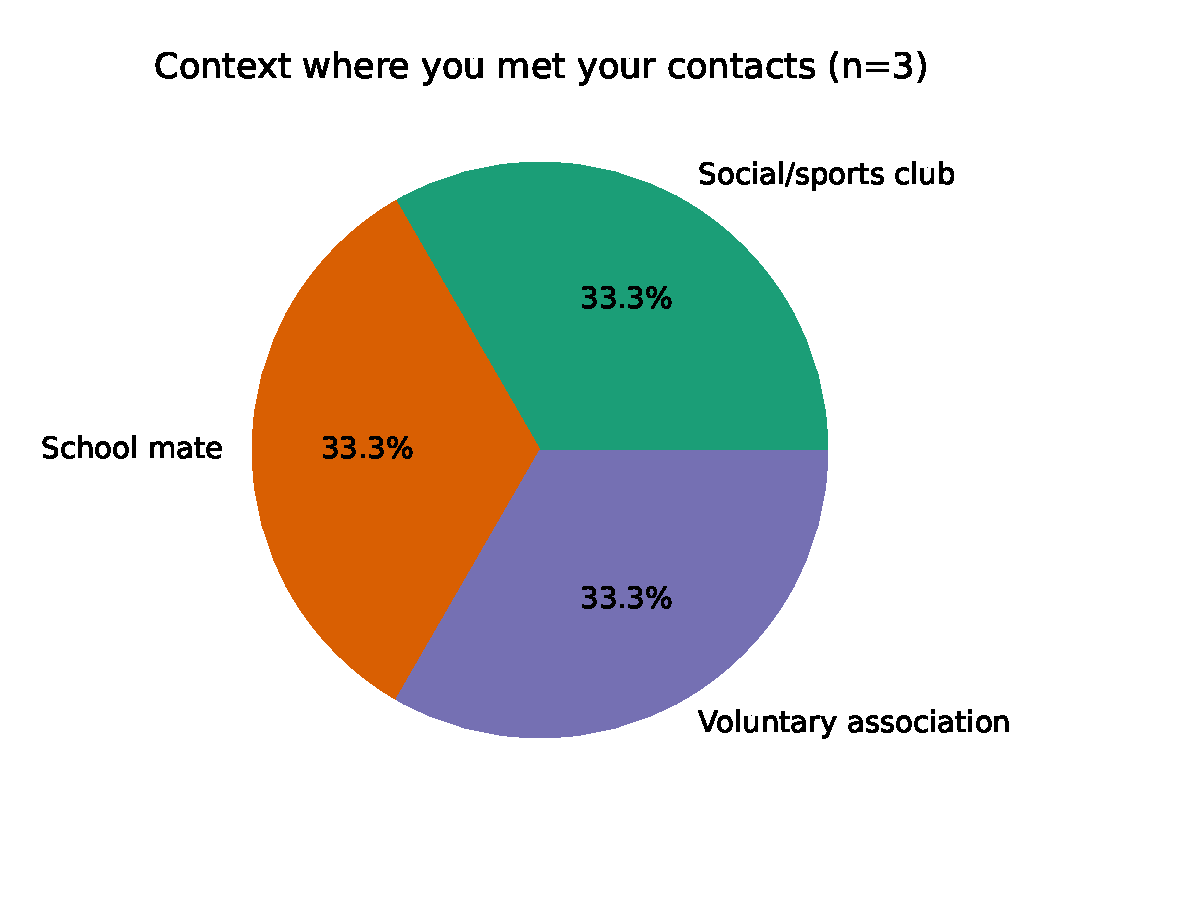
\includegraphics[scale=0.3]{/home/networker/webapps/netwrkr/networker/media/egoreports/3_145721a8-a107-4fd8-a23b-49ab6483bbd0/average/context}}
\hspace{.01in}
\subfloat[Your personal results]{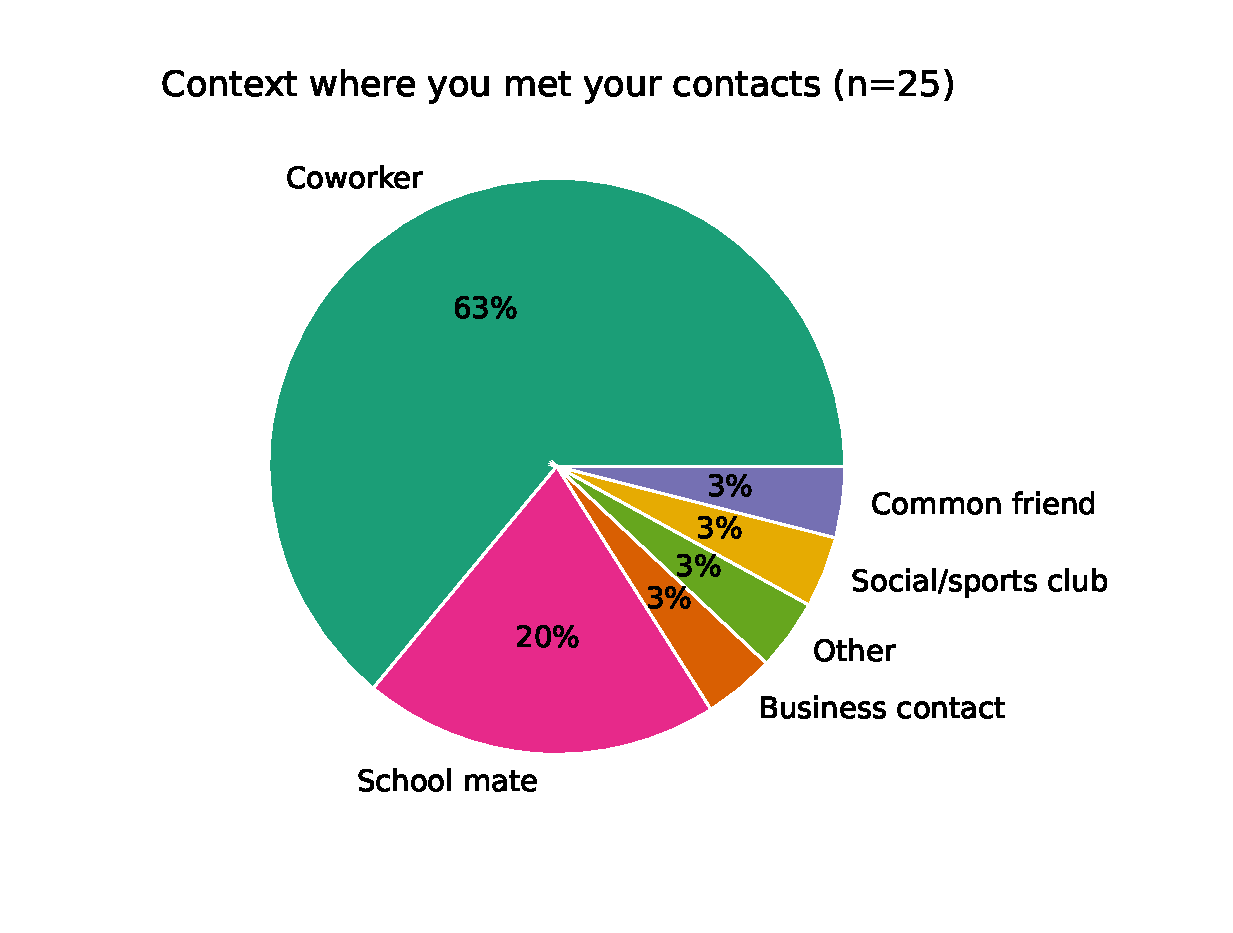
\includegraphics[scale=0.3]{/home/networker/webapps/netwrkr/networker/media/egoreports/3_145721a8-a107-4fd8-a23b-49ab6483bbd0/40dd7ad9-ebed-4bd8-9ab0-034943da2936/gr_context}}
\caption{This chart looks at the origin of your relationships. If most of our contacts come from one single source it is more likely that they will be similar in other aspects too.}
\end{figure}


\section*{Structure of your social network}


As discussed above, social structure is an abstraction to conceptualize the repeated patterns of relations among the people in social groups. A common feature of the structure of social groups is the presence of clusters with dense internal connections, linked by a few ties between clusters. The links that join together dense clusters, and the person that builds those links, are bridges that allow information and resources flow among parts of the organization that would be far apart if there were no such bridging links.

It is usually the case that there is a higher degree of homogeneity within groups than between them. This is because an homophily tendency of individuals to establish relations and bonds with similar others. The person that builds and maintains links that act as a bridge between groups have access to a broader diversity of information, which puts them in a good position for translating domain specific knowledge across groups. Thus, increasing the likelihood of having innovative ideas.


\newpage


\subsection*{Mapping your social network}


You might get a better sense for where you are in the company if you try to position yourself in its social graph. Looking at the connections among people that you are directly connected with can provide useful insight. For instance, you might realize you happen to work as the link between otherwise disconnected others, thus being able to bridge the gap among different groups, receiving knowledge and information from all of them and controlling to some extent the information flow among them.


\begin{figure}[H]
\centering
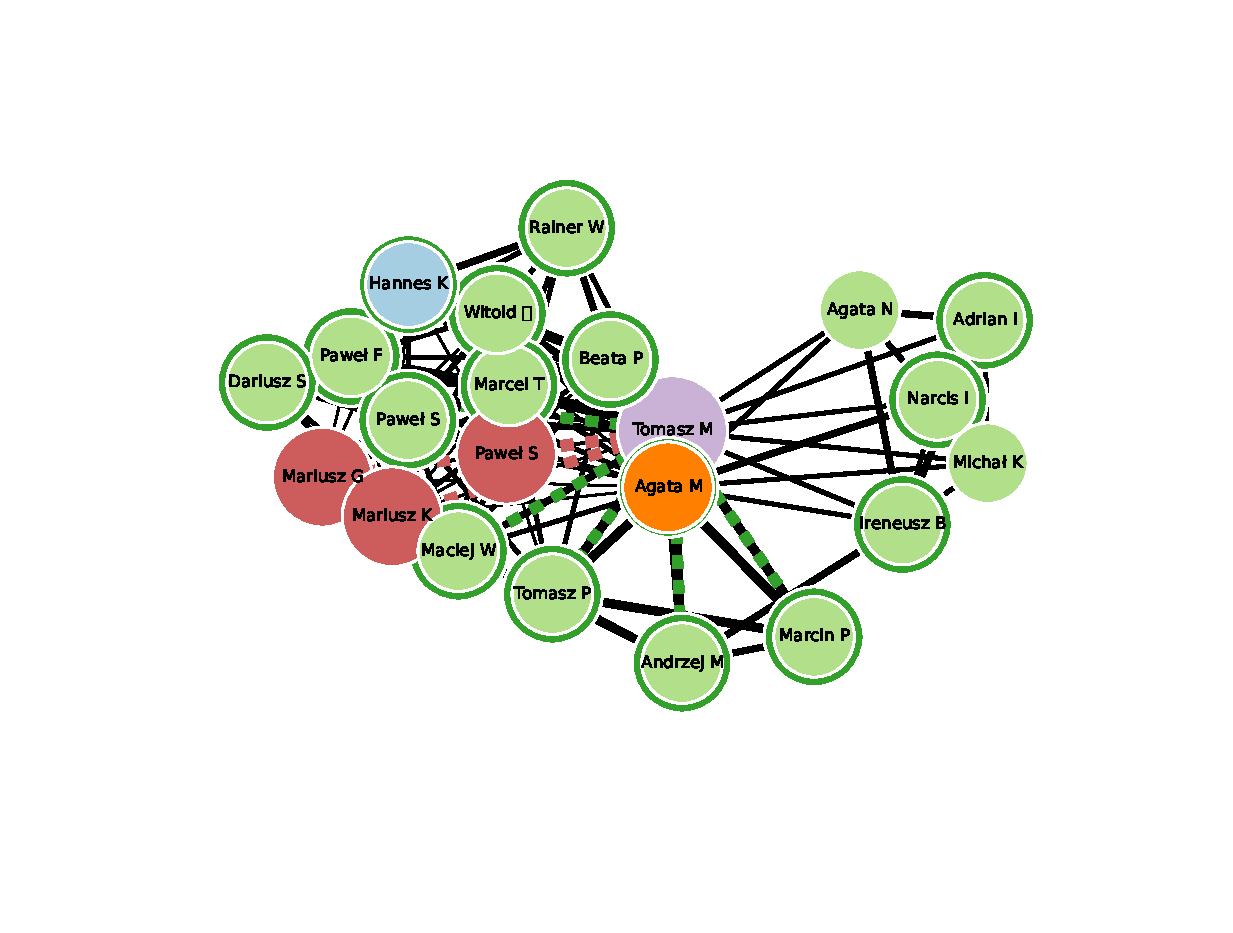
\includegraphics[scale=0.7]{/home/networker/webapps/netwrkr/networker/media/egoreports/3_145721a8-a107-4fd8-a23b-49ab6483bbd0/40dd7ad9-ebed-4bd8-9ab0-034943da2936/egonet_kk}
\caption{In this plot, you and your contacts are depicted as nodes linked through relations of different strength and nature. You are the bigger violet node. The light blue node is your boss. In red you have all the contacts with whom you maintained an adversarial relation (if any). The contacts with the green borders are the ones that you trust. The dashed green edges are the relations that help you the most. Your partner is depicted as an orange node. All other contacts are plotted as smaller light green nodes. The tie width represents the strength of the connection. All adversarial relations are plotted using a dashed red link.}
\end{figure}


\subsection*{Density and centralization of your social network}


Density measures the proportion of actual ties in a network relative to the total number of possible links. A density of 1 means that all potential links in your social network actually exist, and thus everybody in your network know each other. Therefore, the more to the right you are in the centralization/density plot, the less likely that you are acting as a bridge between different groups.

Centralization measures how central is the most central person on your social network, excluding you, in relation to all the other persons. The higher the centralization of your network, the more your network connectivity depends on one or few nodes that are connected with most people around you. Therefore, the likelihood of you actually acting as a bridge between groups in your organization decreases as the centralization of your personal social network increases.

The denser the network, the more all your contacts are connected with one another, and therefore your network is less likely to be centralized. But both high centralized and high density networks are a clear indication that you are not acting as a bridge in your organization, but for different reasons. In dense networks, everybody is linked to everybody else, thus there are no gaps to bridge. In centralized networks, there is another contact, besides you, that is connected to all, or almost all, your other contacts, and thus making your relationships less unique. Persons that act as bridges in actual organizations do have professional networks with low centralization and low or moderate density. Thus, the persons that act as bridges will be positioned in the lower left quadrant of the centralization/density plot.


\begin{figure}[H]
\centering
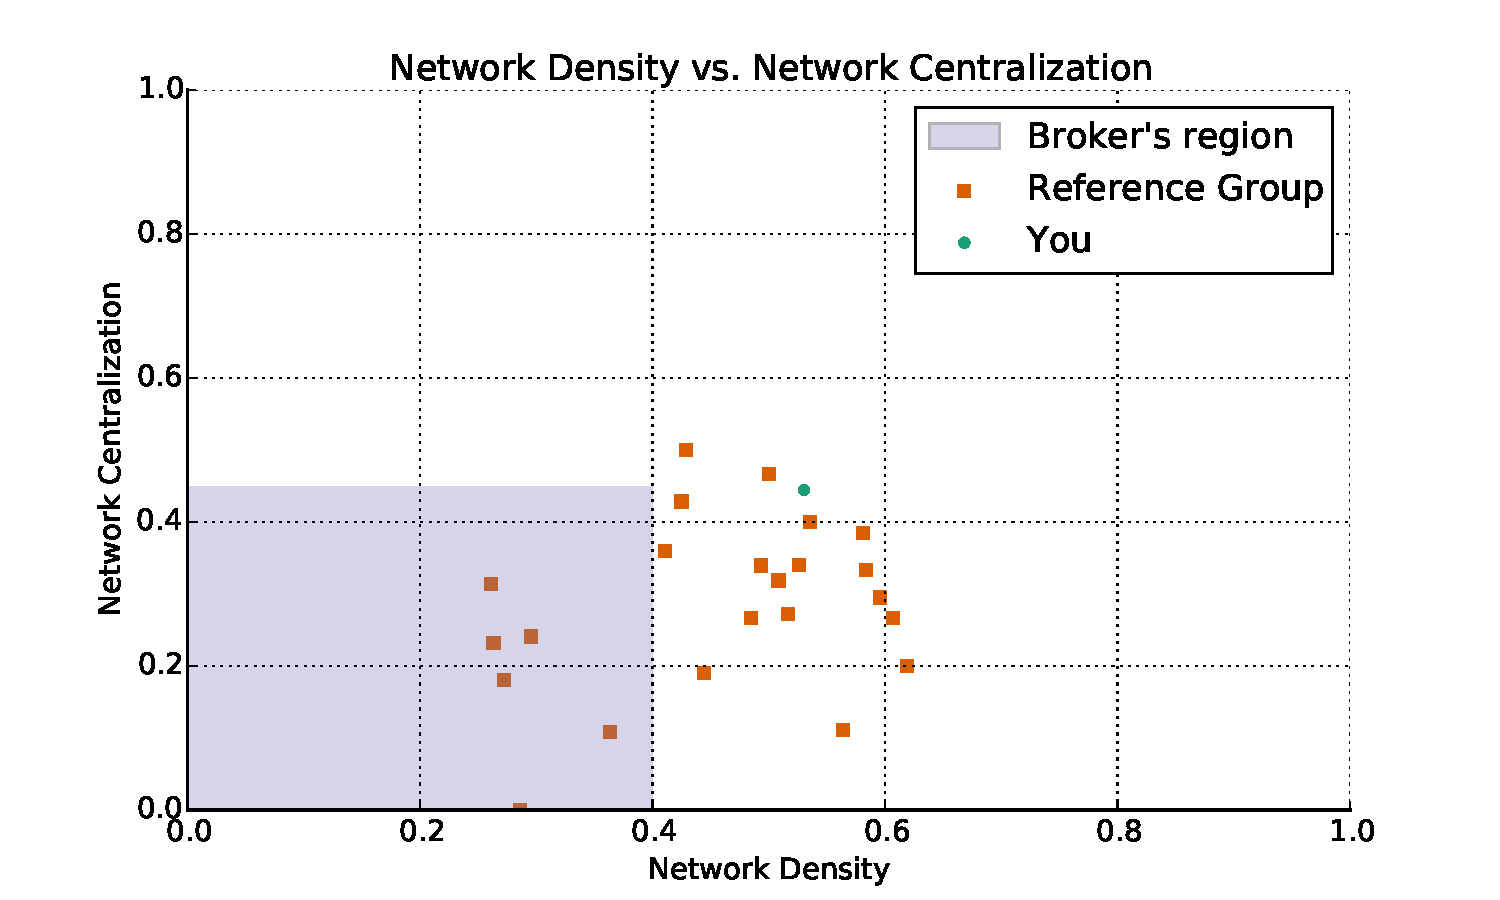
\includegraphics[scale=0.6]{/home/networker/webapps/netwrkr/networker/media/egoreports/3_145721a8-a107-4fd8-a23b-49ab6483bbd0/40dd7ad9-ebed-4bd8-9ab0-034943da2936/density_cent}
\caption{Network centralization vs. network density. The chart above plots both your results and the ones of the other survey respondents using their density and centralization scores. Density measures the proportion of direct ties in a network relative to the total number possible. The higher the centralization of your network, the more your network connectivity depends on one or few nodes that are connected with most people around you. Having a network with high centralization or high density is a clear sign that you are not a broker, as explained in the main text. The highlighted lower left quadrant is the region of social networks with low centrality and low density, these kinds of networks are characteristic of persons that play a broker role.}
\end{figure}


\newpage


\section*{Interesting books on Social Networks}


\begin{itemize}
\item[] Burt, R. 2005. \textbf{Brokerage and Closure}. Oxford University Press.
\item[] Cross, R.L., Thomas, R.J. 2010. \textbf{Driving Results Through Social Networks: How Top Organizations Leverage Networks for Performance and Growth}. Wiley.
\item[] Duan, L., Sheereen, E., and L.M. Weiss. 2014. \textbf{Tapping the power of hidden influencers}. McKinsey Quarterly.
\item[] Ferrazzi, K., and T. Raz, 2005. \textbf{Never Eat Alone: And Other Secrets to Success, One Relationship at a Time}. Doubleday Business.
\item[] Pfeffer, Jeffrey. 2010. \textbf{Power: Why Some People Have It--And Others Don't}. HarperCollins Publishers.
\end{itemize}


\end{document}

